\newpage
\appendix
\renewcommand{\thechapter}{\Asbuk{chapter}}
\chapter{Описание приложения моделирования манипулятора} 
\section{Отличительные особенности} \label{app1start}

Данная программа является отдельным кроссплатформенным приложением, имеющим графический интерфейс. Приложение написано на языке высокого уровня Java. Для построения графического интерфейса был использован фреймворк JavaFX.

Особенности приложения:
\begin{itemize}
\item{Возможность ввода пользователем собственного закона управления для манипулятора в аналитическом виде. Причем, при вводе допускаются как использование элементарных функций, так и интегралов, в том числе, приводящих к уравнениям с запаздыванием (пределы интегрирования зависят от времени)}
\end{itemize}

Патент РФ на программу для ЭВМ №2016616365. Москва, Роспатент, заявка №2016613909. Дата поступления 15.04.2016. Дата государственной регистрации в Реестре программ для ЭВМ 09.06.2016. 

Приложение служит для моделирования движения управляемого трехзвенного манипулятора, анализа управления, времени стабилизации движения манипулятора относительно заданного положения или траектории. Результаты моделирования используются в главе 3 настоящей диссертации.

Для запуска приложения вне зависимости от операционной системы, на которой оно исполняется, необходимо запустить файл manipulator.jar.

На главном экране пользователю предлагается задать параметры системы, такие как геометрические характеристики манипулятора (длины звеньев, расстояния до их центров масс), массы звеньев, начальные положения звеньев, а также законы управления в аналитическом виде. Также присутствует возможность автоматического заполнения заранее подобранными значениями по умолчанию для демонстрации работы программы.

\begin{figure}[h]
\center{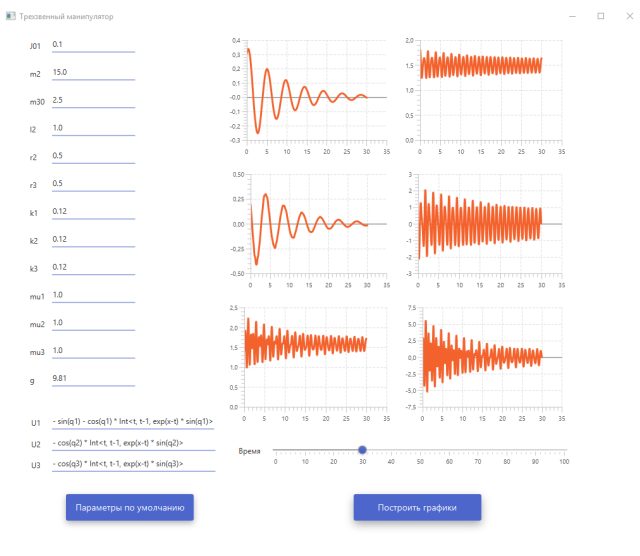
\includegraphics[width=1\linewidth]{program}}
\caption{Основной экран}
\label{ris:modeling}
\end{figure}

В случае возникновения ошибки, программа сообщает о ней, выделяет незаполненные поля в случае недостаточных данных.
\par
\textbf{Задание закона управления манипулятором аналитически}

Для обработки введенных формул используется открытая сторонняя библиотека, позволяющая пользователю вводить элементарные функции. Также библиотека была доработана для того, чтобы иметь возможность распознавать определенные интегралы с переменным верхним или нижним пределом.

Формулы вводятся в поля ввода в качестве строк текста. В формулах допускается использование констант, основных математических операций и параметров системы, таких, например, как массы звеньев, заданные в виде переменных. При обработке формул происходит преобразование текста в объекты языка Java и сохранение в оперативной памяти. Дальнейшие вычисления проводятся с помощью присвоения соответствующим переменным значений, необходимых для работы на текущем шаге. Таким образом, обработка формулы производится только на первых шагах, что положительно сказывается на скорости работы программы.

При необходимости библиотека работы с формулами может быть расширена.

После ввода уравнений управления и параметров системы пользователь нажимает на кнопку построения графиков, после чего программа производит моделирование движения манипулятора и отображает результаты в виде графиков, показывающих соответствующее изменение координат каждого из звеньев, а также изменения скоростей звеньев с течением времени, ограничиваясь максимальным временем, заданным пользователем.

При наборе формулы поддерживаются следующие действия:
\begin{itemize}
\item{основные математические операции (сложение, вычитание, умножения, деление, возведение в степень);}
\item{ввод формул без ограничения на длину;}
\item{ввод без ограничений по количеству вложенных скобок;}
\item{добавление делегированных тригонометрических и алгебраических функций ($sin(t), cos(t), tg(t), ctg(t), exp(t), ln(t)$ );}
\item{ввод определенных интегралов в том числе с подынтегральной функцией и пределов интегрирования в зависимости от времени $t$;}
\item{ввод независимой переменной $t$;}
\end{itemize}
